\subsection{Trapezium}

\subsubsection{Area, knowing base and height}
\begin{figure}[H]
    \centering

    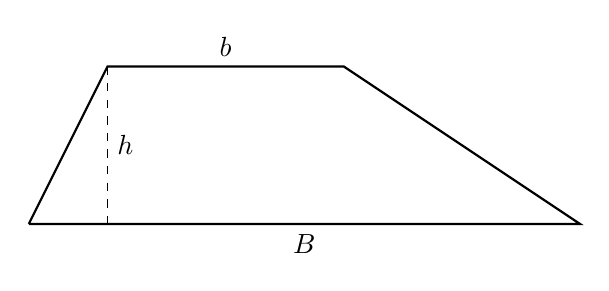
\begin{tikzpicture}
        \coordinate (A) at (0, 0);
        \coordinate (B) at (7, 0);
        \coordinate (C) at (4, 2);
        \coordinate (D) at (1, 2);
        \coordinate (O) at (1, 0);

        \draw[thick] (A) -- node[anchor=north] { $B$ } (B) -- (C) -- node[anchor=south] { $b$ } (D) -- (A);
        \draw[dashed] (D) -- node[anchor=west] { $h$ } (O);

    \end{tikzpicture}
\end{figure}
\[
    A = \frac{(B + b)h}{2}
\]

\subsubsection{Area knowing only sides}

    \begin{figure}[H]
        \centering

        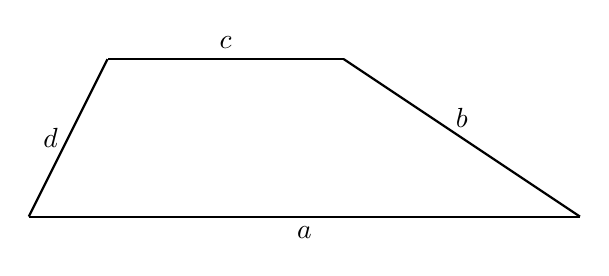
\begin{tikzpicture}
            \coordinate (A) at (0, 0);
            \coordinate (B) at (7, 0);
            \coordinate (C) at (4, 2);
            \coordinate (D) at (1, 2);
            \coordinate (O) at (1, 0);

            \draw[thick] (A) -- node[anchor=north] { $a$ } (B);
            \draw[thick] (B) -- node[anchor=south] { $b$ } (C);
            \draw[thick] (C) -- node[anchor=south] { $c$ } (D);
            \draw[thick] (D) -- node[anchor=east] { $d$ } (A);

        \end{tikzpicture}
    \end{figure}
    \[
        e=\frac{d^2 - b^2+a^2-2ac+c^2}{2a-2c}
    \]

    \[
        h=\sqrt{d^2-e^2}
    \]

    \[
        A=\frac{h(a+c)}{2}
    \]



